\documentclass{llncs}

\usepackage{amsmath}
\usepackage{amssymb}
\usepackage{comment}
\usepackage{url}
\usepackage{listings, tikz}
\usetikzlibrary{positioning,shapes}
\usepackage{verbatimbox}

\newtheorem{Definition}{Definition}
\newtheorem{Theorem}{Theorem}
\newtheorem{Lemma}{Lemma}
\newtheorem{Property}{Property}
\newtheorem{Corollary}{Corollary}
\newtheorem{Proof}{Proof}

\renewcommand{\ttdefault}{pcr}

\lstset{language=Java,
	breaklines=true,
	%basicstyle=\small,
	basicstyle=\ttfamily\footnotesize,
	keywordstyle=\bfseries,
	numbers=left,numberstyle=\scriptsize,
	columns=fullflexible, keepspaces=true,
	%numbers=left,numberstyle=\scriptsize
	%numbers=left,numberstyle=\tiny
	%frame=single
}

\newcommand{\mathword}[1]{{\tt \mathit{#1}}}
\newcommand{\mw}[1]{\mathword{#1}}
\newcommand{\keyword}[1]{\mathsf{#1}}
\newcommand{\kw}[1]{\keyword{#1}}
\newcommand{\ruledef}[3]{ $\frac{\begin{array}[c]{c}{ \rulename{#1}}\\ #2 \end{array}}{\begin{array}[c]{c}#3\end{array}}$}
\newcommand{\ruledefN}[2]{ $\frac{\begin{array}[c]{c} #1 \end{array}}{\begin{array}[c]{c}#2\end{array}}$}
\newcommand{\ruledefX}[2]{ $\begin{array}[c]{c} \rulename{#1}\\ #2 \end{array}$}
\newcommand{\rulename}[1]{{\scriptsize\textsc{[\MakeUppercase{#1}]}}}
\newcommand{\rn}[1]{\rulename{#1}}
\newcommand{\textcode}[1]{\lstinline|#1|}
\newcommand{\tc}[1]{\lstinline|#1|}

\newcommand{\Reducesto}[0]{ \ \Downarrow \ }
\newcommand{\equalson}[1]{ \ \stackrel{#1}{=} \ }
\newcommand{\approxon}[1]{ \ \stackrel{#1}{\approx} \ }
\newcommand{\simon}[1]{ \ \stackrel{#1}{\sim} \ }

\newcommand{\kwnull}[0]{\keyword{null}}
\newcommand{\kwnew}[0]{\keyword{new}}
\newcommand{\kwextends}[0]{\keyword{extends}}
\newcommand{\kwclass}[0]{\keyword{class}}
\newcommand{\kwthis}[0]{\keyword{this}}
\newcommand{\kwif}[0]{\keyword{if}}
\newcommand{\kwthen}[0]{\keyword{then}}
\newcommand{\kwelse}[0]{\keyword{else}}
\newcommand{\kwskip}[0]{\keyword{skip}}

\newcommand\Var{\mathtt{VAR}}
\newcommand\Val{\mathtt{V}}
\newcommand\Obj{\mathtt{OBJ}}

%%% The key relations

\newcommand{\VPT}{\Omega}
\newcommand{\HPT}{\Phi}
\newcommand{\Class}{\mathcal{C}}
\newcommand{\Field}{\mathcal{F}}
\newcommand{\bigO}{\mathcal{O}}
\newcommand{\word}[1]{\langle #1\rangle}
\newcommand{\Nat}{\mathbb{N}}
\newcommand{\less}{\sqsubseteq}
\newcommand{\tflow}{\dashrightarrow}
\newcommand{\hflow}{\rightarrow}
\newcommand{\lhflow}[1]{\stackrel{#1}{\hflow}}

\newcommand\Loc{\mathcal{L}}
\newcommand\Label{\Phi}
\newcommand\set[1]{\{#1\}}
\newcommand\power{\mathcal{P}}
\newcommand\join{\cup}
\newcommand\subtype{\subseteq}

\title{A Relational Static Semantics for Call Graph Resolution}
\author{\today}
\institute{Jinan University}

\begin{document}

\maketitle

\abstract{The problem of resolving virtual method and interface calls in Object-Oriented languages has been a long standing challenge to the program analysis community. In this paper, we propose a new approach called type flow analysis that represent the propagation of type information between program variables by a group of relations without the help of a heap abstraction. We prove that regarding the precision on reachability of class information to variables, our method produces results equivalent to that one can derive from a points-to analysis. Moreover, in practice, our method consumes lower time and space usage, as supported by the experimental results.
}

\section{Introduction}\label{sec:introduction}

For object-oriented programming languages, virtual methods (or functions) are those declared in a base class but are meant to be overridden in different child classes. Statically determine a set of methods that may be invoked at a call site is important to program optimization, from the result of which a subsequent optimization may reduce the cost of virtual function calls or perform inlining if target method forms a singleton set, and one may also remove methods that are never called by any call sites, or produce a call graph which can be useful in other optimization processes.
%
Efficient solutions, such as Class Hierarchy Analysis (CHA)~\cite{Dean1995,Fernandez1995} and Rapid Type Analysis (RTA)~\cite{Bacon1996} and Variable Type Analysis (VTA)~\cite{Sundaresan2000}, conservatively assign each variable a set of class definitions, with relatively low precision. Alternatively, with the help of an abstract heap, one may take advantage of points-to analyses~\cite{andersen94} to compute a set of object abstractions that a variable may refer to, and resolve the receiver classes in order to find associated methods at call sites.

The purpose of the conservative analyses, such as CHA, RTA and VTA, is to provide an efficient way to resolve calling edges, which usually executes linear-time in the size of a program, by focusing on the types that are collected at the receiver. For instance, let $x$ be a receiver with declared class $A$, then at a call site $x.m()$, then CHA will draw a call edge from this call site to method $m()$ of class $A$ and every definition $m()$ of a class that extends $A$. In case class $A$ does not define $m()$, a call edge to the nearest parent class that defines $m()$ will also be included. For $x$ a receiver with declared interface $I$, then CHA will draw a call edge from this call site to every method of name $m()$ defined in class $X$ that implements $I$.
We write $CHA(x,m)$ for the set of methods that are connected from call site $x.m()$ as resolved by  Class Hierarchy Analysis (CHA).
Rapid Type Analysis (RTA) is an improvement from CHA which resolves call site $x.m()$ to $CHA(x,m)\cap inst(P)$, where $inst(P)$ stands for the set of methods of classes that are instantiated in the program.

\begin{figure}[t!]
\begin{minipage}[t]{0.5\linewidth}
\centering
\begin{verbbox}
class A{
    A f;
    void m(){
        return this.f;
    }
}

class B extends A{}

class C extends A{}
\end{verbbox}
\theverbbox
\end{minipage}
\begin{minipage}[t]{0.5\linewidth}
%\center
\centering
\begin{verbbox}
1:  A x = new A();  //O_1
2:  B b = new B();  //O_2
3:  A y = new A();  //O_3
4:  C c = new C();  //O_4
5:  x.f = b;
6:  y.f = c;
7:  z = x.m();
\end{verbbox}
\theverbbox
\end{minipage}
\caption{An example that compares precision on type flow in a program.}\label{figure:example}
\end{figure}

Variable Type Analysis (VTA) is a further improvement from RTA. VTA defines a node for each variable, method, method parameter and field. Class names are treated in a similar way as to variables, and propagation of value between variables work in the way of value flow.
As shown in Figure~\ref{figure:vta}, the statements on line $1-4$ initialize type information for variables $x$, $y$, $b$ and $c$,
and statements on line $5-7$ establish value flow relations. Since both $x$ and $y$ are assigned type $A$, $x.f$ and $y.f$ are both represented by node $A.f$, thus the set of types reaching $A.f$ is now $\set{B,C}$. (Note this is a more precise result than CHA and RTA which give $\set{A,B,C}$ as the set of types reaching $A.f$.)
Since $A.m.this$ refers to $x$, $this.f$ inside method $A.m()$ now refers to $A.f$. Therefore, through $A.m.return$, $z$ receives  $\set{B,C}$ as its final set of reaching types.

\begin{figure}[t!]%%[ht]
\begin{tabular}{cc}

\begin{minipage}[h]{0.5\linewidth}
\begin{tabular}{|c|c|}
  \hline
  \textbf{Statement} & \textbf{VTA fact} \\
   \hline
  \hline
  % after \\: \hline or \cline{col1-col2} \cline{col3-col4} ...
  $A\ x = \kwnew\ A()$ & $x\leftarrow A$ \\ \hline
  $B\ b = \kwnew\ B()$ & $b\leftarrow B$ \\ \hline
  $A\ y = \kwnew\ A()$ & $y\leftarrow A$ \\ \hline
  $C\ c = \kwnew\ C()$ & $c\leftarrow C$ \\ \hline
  $x.f = b$ & $A.f\leftarrow b$ \\ \hline
  $y.f = c$ & $A.f\leftarrow c$ \\ \hline
   & $A.m.this\leftarrow x$ \\
  $z = x.m()$  & $A.m.return\leftarrow A.f$ \\
   & $z\leftarrow A.m.return$\\
  \hline
\end{tabular}
\caption{VTA facts on the example}\label{figure:vta}
\end{minipage}
&
\begin{minipage}[h]{0.5\linewidth}
\centering
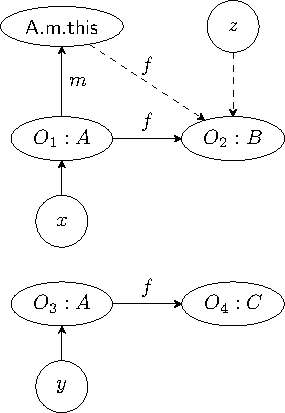
\includegraphics[width=3.5cm]{points-to.pdf}
\caption{Points-to results on the example}\label{figure:points-to}
\end{minipage}
\end{tabular}
\end{figure}

The result of a context-insensitive subset based points-to analysis~\cite{andersen94} creates a heap abstraction of four objects (shown on line $1-4$ of Figure~\ref{figure:example} as well as in the ellipses in Figure~\ref{figure:points-to}). These abstract objects are then inter-connected via field store access defined on line $5-6$. The derived field access from $O_1.m.this$ to $O_2$ is shown in dashed arrow. By return of the method call $z=x.m()$, variable $z$ receives $O_2$ of type $B$ from $O_1.m.this.f$, which gives the most precise type for variable $z$.

From this example, one may conclude that the imprecision of VTA in comparison with points-to analysis is due to the over abstraction of object types, such that $O_1$ and $O_3$, both of type $A$ are treated under the same type. However, points-to analysis often requires to construct a heap abstraction, which brings in extra information especially in the case when we are only interested in the type of a variable.

\begin{figure}[t!]
\[\dfrac{\dfrac{\dfrac{z=x.m(), \mbox{\textsf{[call]}}}{A.m.this.f\less A.m.return}\quad
  \dfrac{\dfrac{z=x.m(), \mbox{\textsf{[call]}}}{x\less A.m.this}\quad\dfrac{x.f=b, \mbox{\textsf{[store]}}}{x\lhflow{f}b}}
  {A.m.this\lhflow{f}b}\mbox{, \textsf{[load]}}}{b\less A.m.return}\quad
  \dfrac{z=x.m(), \mbox{\textsf{[call]}}}{A.m.return\less z}}{b\less z}\]
\caption{Type Flow Analysis for variable $z$ in the example}\label{fig:tfa}
\end{figure}

In this paper we introduce a relational static semantics called Type Flow Analysis (TFA) on program variables and field accesses. Different from VTA, besides a binary value flow relation $\less$ on the variable domain $\Var$, where $x\less y$ denotes all types that flow to $x$ also flow to $y$, we also build a ternary field store relation $\rightarrow\ \subseteq\Var\times\Field\times\Var$ to trace the \emph{load} and \emph{store} relationship between variables via filed accesses. This provides us more ways to enlarge the relations $\less$ and $\rightarrow$. For example given $x\lhflow{f}y$ and $x\less z$, we can derive $z\lhflow{f}y$.

Taking the example from Figure~\ref{figure:example}, we are able to collect the store relation $x\lhflow{f}b$ from line $5$. Since $x\less C.m.this$, we derive $C.m.this\lhflow{f}b$, which together with $C.m.this.f\less z$, further derives $b\less z$. Therefore, we assign type $B$ to variable $z$. The complete reasoning pattern is depicted in Figure~\ref{fig:tfa}. Nevertheless, one cannot derive $c\less z$ in the similar way.

%%% contributions with %%% discussion on context-sensitivity
We have proved that in the context insensitive inter-procedural analysis, the TFA is as precise as subset based points-to analysis regarding type related information. Since points-to analysis can be enhanced with context-sensitivity on both variables and objects (e.g.,~\cite{Milanova2005,Smaragdakis11,Tan16}), our type flow analysis only requires to consider context on variables, which is left for future work. The context-insensitive type flow analysis has been implemented in SOOT~\cite{soot}, and has been tested on a collection of benchmark programs from specjvm2008 and DaCapo. (Need more citations here, and brief the experimental results.)

\section{Type Flow Analysis}\label{sec:type-flow-analysis}

We define a core calculus in Figure~\ref{fig:syntax} consisting of most of the key Object-Oriented language features.
A program is defined as a code base $\overline{C}$ (i.e., a collection of class definitions) with statement $s$ to be evaluated.
To run a program, one may assume that $s$ is the default (static) entry method with local variable declarations $\overline{D}$,
similar to e.g., Java and C++,
<<<<<<< HEAD
which may differ in specific language designs. 
=======
which may differ in specific language designs.
>>>>>>> 758c8f4a6a400c0f32c935d69acb909b4c579804
%% to consider dynamic semantics later: Let $S$ and $H$ be the runtime stack and heap, where $S:\Var\rightarrow \Val$maps local variables to values and $H:\Val\rightarrow \Obj\cup\set{\kwnull}$ maps values to objects.
Two auxiliary functions are given. Function $fields$ maps class names to its fields, and $class$ provides types (or class names)
for objects.
Given class $c$, if $f\in fields(c)$, then $type(c,f)$ is the defined class type of field $f$ in $c$. Similarly, give an object $o$,
if $f\in fields(class(o))$, then $o.f$ may refer to an object of type $type(class(o),f)$, or an object of any of its subclass at runtime.
%Sometimes we mix-use the terms \emph{type} and \emph{class} in this paper when it is clear from the context.

\begin{figure}[!htbp]\centering
	\begin{tabular}[c]{lll} %\hline
		%Classes&$C$&$::=$&$\kwclass\ c\ [\kwextends\ c] \ \{\overline{c\ f};\ \overline{M}\}$\\
		%Methods&$M$&$::=$&$c\ m(\overline{c\ x}) \ \{\overline{c\ x};\ e\}$\\
		$C$&$::=$&$\kwclass\ c\ [\kwextends\ c] \ \{\overline{F};\ \overline{M}\}$\\
        $F$&$::=$&$c \ f$\\
        $D$&$::=$&$c \ z$\\
		$M$&$::=$&$m(x) \ \{\overline{D}; s\}$\\
		$s$&$::=$&$e\mid x{=}\kwnew \ c\mid  x {=} e \mid x.f{=}y $\\
		&&$ \mid \kwif \ x \ \kwthen \ s \ \kwelse \ s \ |\ s;s$\\
		$e$&$::=$&$ \kwnull\mid x \mid x.f \mid x.m(y) $\\
        $prog$&$::=$&$\overline{C};\overline{D}; s$\\
	\end{tabular}
	\caption{Abstract syntax for the core language. \label{fig:syntax}}
\end{figure}


\section{Optimization}\label{sec:minimization}



\section{Experiment}\label{sec:experiment}


\section{Related Work}\label{sec:related-work}



\bibliographystyle{plain}
\bibliography{literature}
\end{document}
<<<<<<< HEAD
=======

>>>>>>> 758c8f4a6a400c0f32c935d69acb909b4c579804
